\section{Scale Lab}
We can hear a wide range of frequencies. Usually we don't use all the audible frequencies to make music, we select a discrete set of them to determine the pitch of each tone, and we call this set of frequencies a scale. Depending on the choice of the scale, we will be able to play some combinations. Interestingly, humans find that some pairs of frequencies sound ``good'' together (consonant), while others sound ``bad'' (dissonant). This is a physiological and psychological phenomenon still under debate and being actively researched today. This preference has determined the choice of scales and the practice of music since the beginning of its history.

In this exhibit, we explore the creation of scales and their properties. Along the gray horizontal line all the frequencies are represented. The markers represent frequencies selected for the particular  scale, and they are connected to the keyboard by the blue lines that allows us to play them.

\begin{figure}[h]
\centering
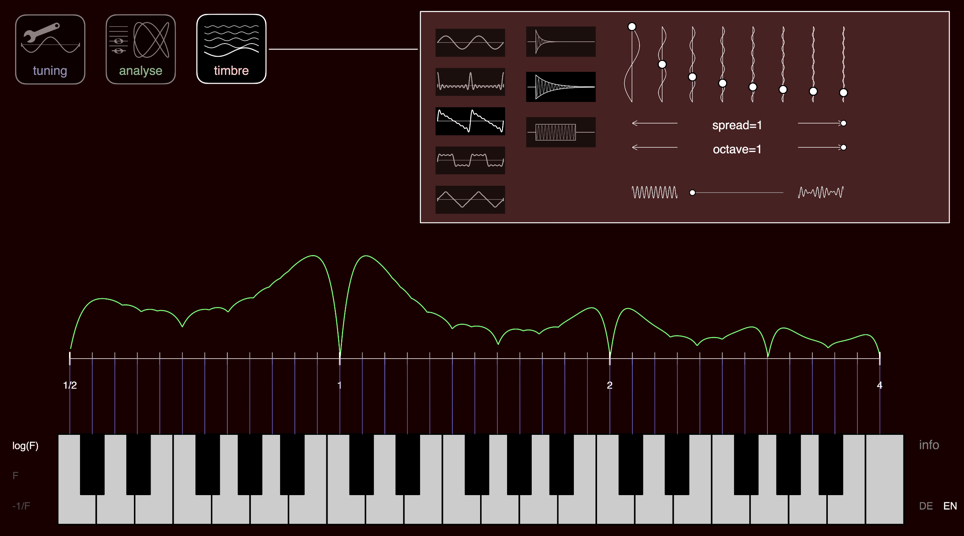
\includegraphics[width=0.9\textwidth]{ScaleLab_1}
\end{figure}

\subsection{The Tools}
A set of three toolboxes helps us influence the characteristics of a tone (timbre), the selection of the pitches for the scale (tuning) and to analyze properties of tones and combinations of tones (analyze).

\subsubsection{Tuning}
You can choose Western scales (with different tunings), two oriental scales (Raga, Gamelan), and two tools to generate scales (one with a step-generator and another with free pointing).

\subsubsection{Analyze}
The analyze toolbox contains the implements that help you to understand the scale and/or tuning you selected.

\subsubsection{Waveform}
This is the signal you hear, the movement of the speaker's membrane (and your eardrum) over time. Choose a sine as timbre and press one key to hear a pure frequency. Play two or more to see the combined waves (addition). Choose a different timbre (composed of many frequencies) to see its waveform and hear the difference.

\subsubsection{Lissajous}
This curve is drawn by a moving point with an x-coordinate given by the oscillation determined by the first key stroke, and a y-coordinate given by the second key stroke. This works better with a pure sine waveform as timbre, but it also creates very interesting curves for more complicated timbres. Simple ratios between the two frequencies give simpler figures, which are also the more ``consonant''.

\subsubsection{Ratio}
You can see the proportions between the (fundamental) frequencies of the notes played. Check the different scales to see how simpler ratios are related to consonant intervals.

\subsubsection{Dissonance curve}
Real instruments don't produce a single frequency, instead many of them simultaneously (spectrum). Thus consonance or dissonance depends on the interaction of the two groups of frequencies. This curve (based on a concept from Helmholtz) attempts to measure dissonance (badness) of every tone with respect to the fixed middle C tone, and it varies when the timbre is changed. Note that dissonance is at a minimum for an octave jump or fifth and major third jumps.

\subsubsection{Timbre}
A musical tone produced by an instrument is not usually a single pure frequency, but a mixture of different frequencies with different intensities (spectrum). This toolbox allows the selection of  some predefined spectra as well as defining one yourself by adjusting the sliders. All scales, tuning settings, and analysis performed with other toolboxes is strongly affected by the timbre of the instrument you choose to play.

\subsection{Backgrounds and Experiments}
The following pages describe concepts and experiments that can be experienced using the Scale Lab exhibit.

\subsubsection{Beating}
If two frequencies are close, an exciting and fundamental acoustic phenomenon occurs: the sound seems to periodically increase and decrease in volume... and it actually does. There are two ways to explain this effect. One is more qualitative: assum
e you have two frequencies one of 100 vibrations per second and one of 101 vibrations per second. At every moment of time these two waves will sum up. If the trough of one wave meets the peak of the other the two signals will cancel out. If a peak meets another peak the intensity is double that of the single signal.

\begin{figure}[h]
\centering
\begin{tikzpicture}
\scriptsize
\node at (0,0) {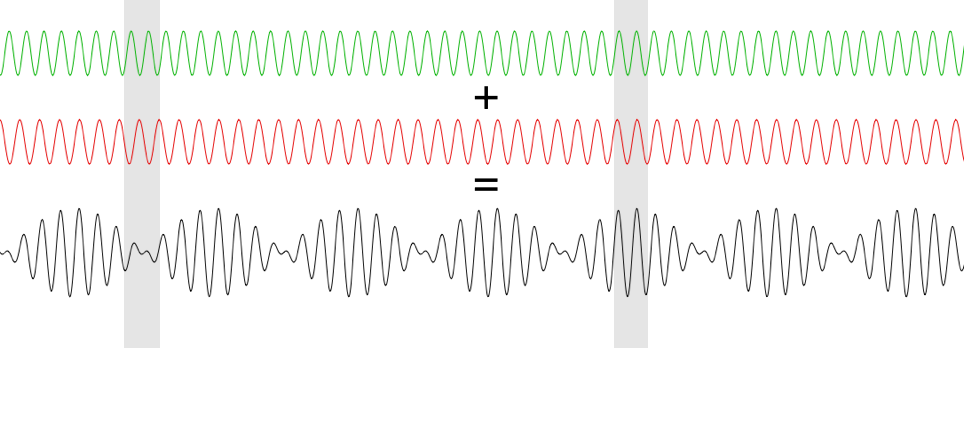
\includegraphics[width=0.9\textwidth]{ScaleLab_3_nolabels} };
\node at (-3.86,-1.6) [align=center, anchor=north]
    {Mountain meets valley, \\ signal gets silent.};
\node at (1.73,-1.6) [align=center, anchor=north]
    {Mountain meets mountain, \\ signal gets loud.};
%\draw (-3.86,-1.6) circle [radius=0.5mm];
%\draw (1.73,-1.6) circle [radius=0.5mm];
\end{tikzpicture}
\end{figure}

The second way to think about it is more quantitative. There is a nice trigonometric formula that describes what happens if two sine waves of different frequencies $f_1$ and $f_2$ are added:
$$\sin(f_1 \cdot t) + \sin(f_2\cdot t) = 2 \sin\left( \frac{f_1+f_2}{2}\cdot t\right) \cdot \cos\left( \frac{f_1-f_2}{2}\cdot t\right) .$$
The resulting wave can be considered as a signal vibrating in the average frequency (the sin part of the right hand equation) and modulated by a low frequency signal depending on the difference of the frequencies (the cos part of the right hand equation). If the frequencies are close together this will be heard as low frequencies change in intensity.

\paragraph{Experiment:} Go to timbre and select a pure sine wave. Then use multi-touch on the central horizontal frequency line to create two nearby tones by using two fingers. Listen to the beating. The closer the frequencies are the slower the beating. If you move them far apart at some point the beating gets so fast that you perceive it as a rough dissonance. Moving them even further apart they will be perceived as two different tones. Analyze this using Lissajous or wave to actually see the beating.

\paragraph{Music:} Slow beating sounds like a bit like a vibrato, it makes a tone sound richer and a bit more organic. This is the reason why in several instruments beating is taken as part of the sound generation process. In a piano the high frequency notes usually have two or three strings. These strings are slightly detuned with respect to each other, resulting in an organic and rich tone. Also a Musette register on an accordion has two slightly detuned vibrating metal tongues generating a vibrato sound.

\subsubsection{Sound from Overtones}
The timbre settings of Scale Lab allow for much more than just simple sine waves, you can combine sine waves to generate a complex sound. The sliders in the timbre box allow you to add multiples of the base frequency. If the spread slider is set to 1 these are really the integer multiples $f$, $2f$, $3f$, $4f$, $5f$, $6f$, $7f$, $8f$. of the base frequency. Fourier synthesis implies that any periodic signal can be generated by a weighted sum of sine waves of the above type. You would need infinite summands to replicate a perfect signal, but the eight frequencies offered by Scale Lab are already pretty precise.

\begin{figure}
\centering
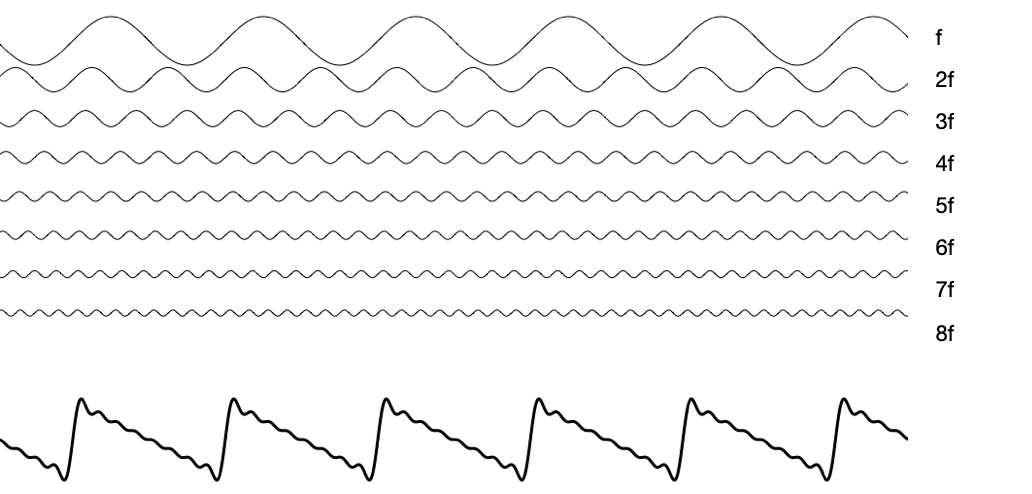
\includegraphics[width=0.9\textwidth]{ScaleLab_5}
\caption*{This illustrates how the summation of overtones with intensity 1, 1/2, 1/3, 1/4, ... results in a sawtooth-like periodic function.}
\end{figure}

\paragraph{Experiment:}
Go to timbre and experiment with the different presets for wave forms (buttons on the left). Move the individual sliders of the timbre overtones to monitor how the sound changes. Use the ``analyze tool'' to see the shapes of the waves you generated.

\paragraph{Music:}
As a matter of fact, the sound of many instruments (in particular strings, brass or woodwind instruments is nicely approximated by decomposing the sound into a composition of overtones. This has to do with the specific physics of the instruments.

\begin{figure}
\centering
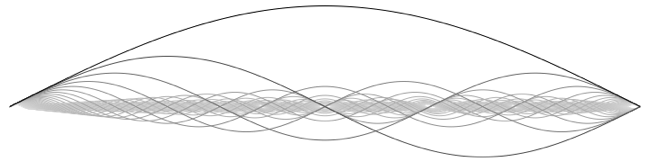
\includegraphics[width=0.9\textwidth]{ScaleLab_6}
\caption*{The image shows the partial waves of an ideal vibrating string. They correspond exactly to the overtones, resulting in a sound that can be very well modeled by this approach.}
\end{figure}


\subsubsection{Spread partials}
The world is not an ideal laboratory. Physics is dirty and sounds are not perfect sums of overtones. As a matter of fact, most instruments create sounds where frequencies of the higher vibrations do not perfectly match overtones. For instance the fact that a string is not infinitely thin results in a certain spread of the overtones. The thicker the vibrating material gets the more extreme is the deviation form the ideal overtone series. The spectrum of a church bell is substantially different from an overtone series. This is not a bad thing. It makes sounds richer, more individual, or more characteristic. Below you see what happens if the overtone spectrum is replaced by a spread spectrum where the frequencies follow the law
$$1^af, 2^af, 3^af, 4^af, 5^af, 6^af, 7^af, 8^af$$
for a small exponent $a$. Observe that the resulting sum of the partials (this is the correct name here) shows ever changing behavior in the resulting sound curve and is no longer periodic. The resulting sound is rich and organic.

\paragraph{Experiment:}
In the  Scale Lab Timbre Box there is a slider called spread right under the overtone sliders. Play with the slider to experiment with spread and compressed spectra. Listen how the sound changes even if you only add a very slight spread. Analyze the resulting sound with the wave tool to see how the wave forms change. How do intervals sound? What is the difference between a small and a large spread? Between a spreading and a compression of the spectrum? There is a whole world to be discovered.


\subsubsection{Dissonance curves}
As soon as two tones (with a certain spectrum of partials) are played together our brain starts to categorize the intervals in a range
A between pleasant sounding (consonant) and not-so-nice sounding (dissonant). One can think of the entire art of music as the art of creating the right tension between consonance (to please people) and dissonance (to make it interesting). Different epochs and cultures have different opinions at what is good style, but the global topic remains.

\begin{figure}[h]
\centering
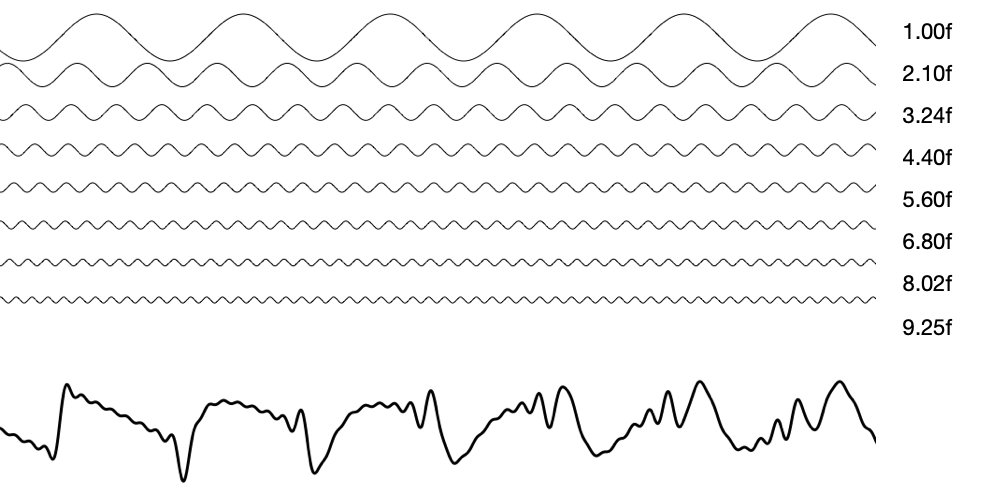
\includegraphics[width=0.9\textwidth]{ScaleLab_7}
\caption*{There is another interpretation of the richness of sound that arises. Since the partials do not perfectly match the overtones as soon as intervals are played, there is a substantial and quite irregular beating of the higher frequencies.}
\end{figure}

Already around 1870 Hermann von Helmholtz developed a mathematical theory of consonance and dissonance. The idea behind it is brilliant and simple. Since whenever two tones are played together many partials sound at the same time, one has to sum up the dissonances between all pairs of involved sine waves to get the dissonance of the entire sound. Therefore, he reduces the question of dissonance of complex sounds to the question of dissonance between sine waves. (One might ask if this is a reasonable assumption but at least it is a good starting point). However, what is the dissonance between two sine waves? Here we need empirical data. It turns out that if sine waves with more or less of identical frequency are not perceived as dissonant. A small, low frequency beat even slightly pleases. However, as soon as the beating becomes too fast it is perceived as rough and dissonant. This effect is particularly strong for beats between 10 and 25 beats per second, after that the effect decreases again. If the tones are too far apart they are just heard as two sine waves. Below you see a dissonance curve of a sine wave referring to a middle C.

\begin{figure}[h]
\centering
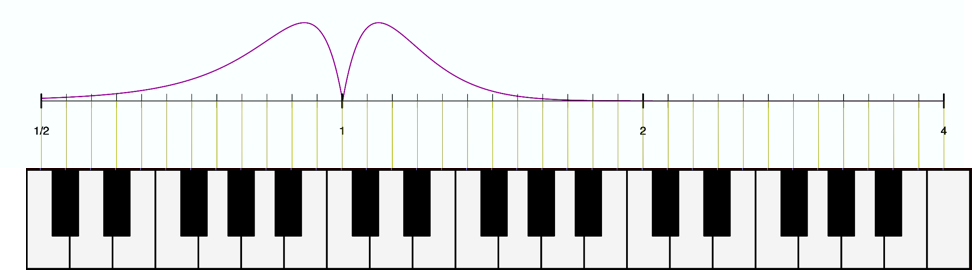
\includegraphics[width=0.9\textwidth]{ScaleLab_9}
\end{figure}

Things get interesting as soon as the spectra become complicated. The next picture shows the dissonance curve resulting from a rich overtone spectrum. Dissonances between overtones of the two tones generate characteristic maxima and minima of that curves. Notice that for the usual perfect overtones you get minima at the octave, the fifth, the quarter and the third.

\begin{figure}[h]
\centering
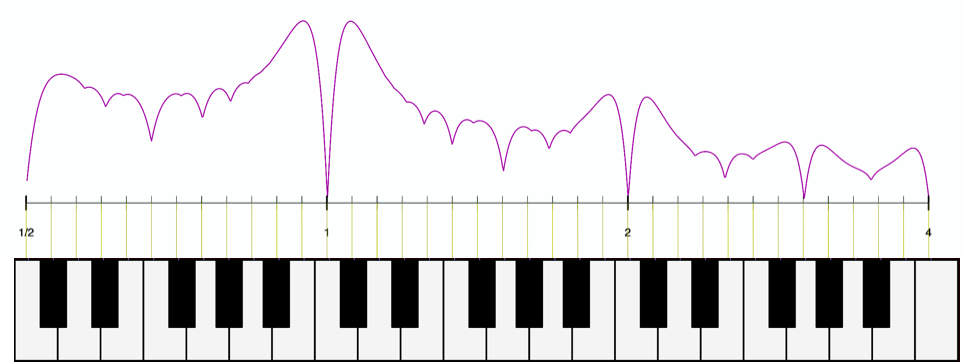
\includegraphics[width=0.9\textwidth]{ScaleLab_10}
\end{figure}

\paragraph{Experiment:}
Start the dissonance curve analyzer and play intervals with the central C. Play with different timbres and experiment with different intervals, Does the prediction meet you personal perception?


\subsubsection{Dissonance and spread partials}
What happens if we study the dissonance behavior of a spectrum with spread partials? The dissonance behavior is very much determined by the dissonance between the overtones or partials. Consequently, as soon as the partials are ``out of place'' you get a new dissonance behavior.

The following image shows what happens to a slightly spread spectrum ($a=1.08$):

% \begin{figure}[h]
% \centering
% 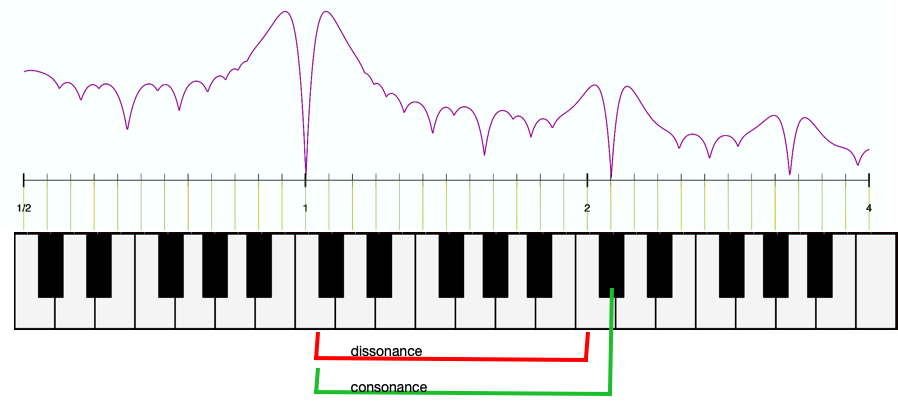
\includegraphics[width=0.9\textwidth]{ScaleLab_11}
% \end{figure}

\begin{figure}[h]
\centering
\begin{tikzpicture}
\scriptsize
\node at (0,0) {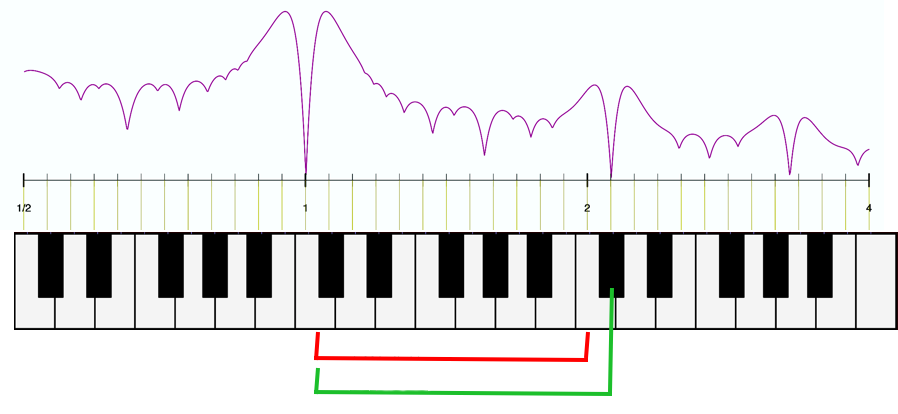
\includegraphics[width=0.9\textwidth]{ScaleLab_11_nolabels} };
\node at (-1,-1.65) [align=left, anchor=west]
    {dissonance};
\node at (-1,-2.08) [align=left, anchor=west]
    {consonance};
%\draw (-1,-2.05) circle [radius=0.5mm];
\end{tikzpicture}
\end{figure}

For a musician used to our classical tone system the result might be a little bit shocking. Suddenly intervals that usually sound consonant (like the octave) sound heavily dissonant. While others that usually sound very dissonant (like the small ninth between C and c$\sharp$) sound as sweet as sugar.

Therefore, instruments that generate a spread or compressed spectrum require a different kind of scale. Or to put it differently, our Western tonal system is heavily influenced by the fact that we have strings, brass and woodwinds.

There is an amazing cure to fix the dissonant sounding octaves: Spread the frequencies of your scale as well! After that an octave is no longer an octave, but it sounds like one.

\begin{figure}[h]
\centering
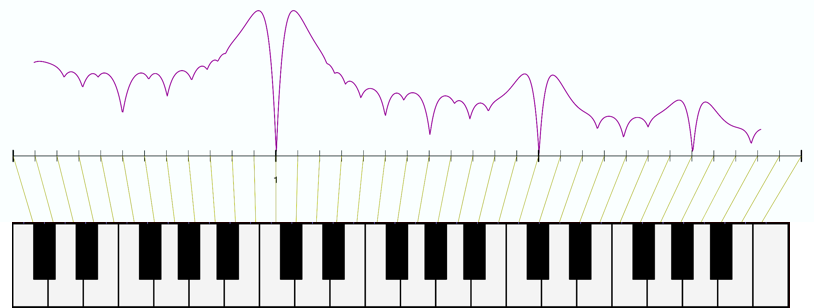
\includegraphics[width=0.9\textwidth]{ScaleLab_12}
\end{figure}

\paragraph{Experiment:}
The following experiments may be eye-opening. Start the dissonance curve analyzer and play intervals with the central C. Experiment with the spread of the spectrum and with the spread of the octave. Spreading both by the same amount gets you close to the usual tonal experience.

\paragraph{Music:}
In some instances, it may be good practice to spread scales. If you design the bells for a church tower adapting the scale to a spectrum is a good idea. Even an ordinary piano sounds more brilliant if the octaves are slightly spread. However, a piano with slightly spread scales will make it difficult to play along with other instruments. Music is full of compromises.

\subsubsection{Western Tuning Systems}
We have seen that the timbre and the frequencies of the partials heavily influence the dissonance behavior of intervals. As a consequence, the selection of pitches (the scale) used on an instrument should depend on the sound characteristics of the instrument. Western culture instruments (harps, pianos, flutes, trumpets, have a close to perfect spectrum in the sense that the partials are very close to the theoretical overtones. Therefore, frequency ratios of 2 : 1 (octave), 3 : 2 (fifth), 4 : 3 (fourth), 4 : 5 (major third) and 6 : 5 (minor third) result in relatively consonant intervals (in this order with decreasing strength).

It turns out that fifths, fourths (Gregorian music), then later thirds (baroque) and even later more dissonant intervals (impressionists, expressionists) entered the musical language in the Western culture.

What is a good selection of pitches for such music? What are good scales? Answering these questions in depth could easily fill a one year university class. We will only scratch the surface.


12-Tone system: Current Western music culture systems of twelve tones within an octave are predominant. The reason for this is in a sense mathematical. Stacking 12 perfect fifths nearly hits stacking seven octaves. Or in formulas:
$$\left( \frac{3}{2}\right)^{12} = 129.7463 \ldots \approx 2^7 = 128 .$$
The 12 steps are the first time this stacking procedure comes close to an octave relation. If one wants a tonal system that is focused around octaves and fifth, then 12 tones are a good start.

Unfortunately, this relation is not perfect and this is where the entire story of tuning systems begins: one has to make compromises and different epochs resolved this tension in different ways.

\begin{figure}[h]
\centering
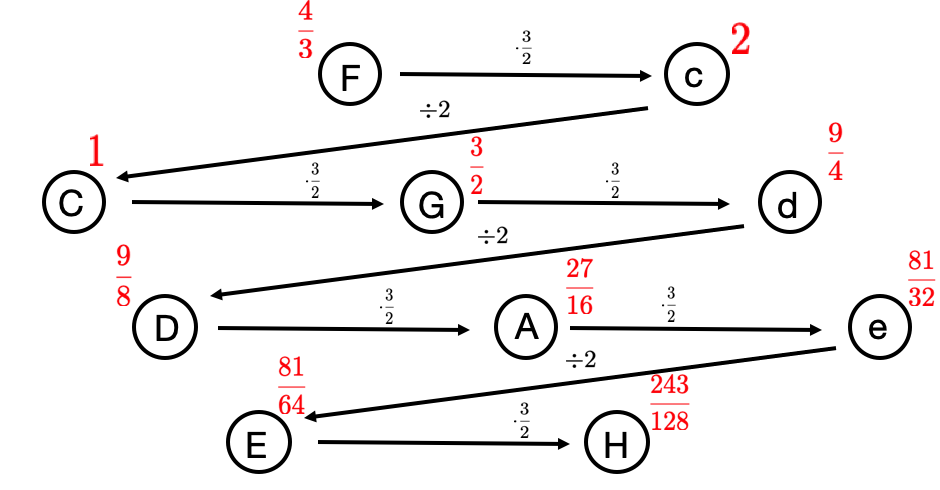
\includegraphics[width=0.7\textwidth]{ScaleLab_14}
\caption*{Pythagorean tuning}
\end{figure}


Pythagorean Tuning: Let us start with Pythagorean tuning, which focuses around the idea of having as many perfect fifths as possible. Focus on the seven tones of our C major scale and see what happens. We label the tones by frequency ratios with respect to C and divide by two (drop an octave) every time we become greater than two. The following diagram shows the frequency ratios of notes in the Pythagorean scale and how they are derived.

All fifths and octaves in this tuning are perfect. However, notice that the note E gets assigned a frequency value of 81/64. This is not a perfectly tuned major third, the perfect third would be 5/4 = 80/64.

Thus the Pythagorean third is off by a factor of 81/80 from the perfectly tuned third. Most likely the Pythagoreans would not have cared a lot since thirds only became an important interval in music over 1500 years later. As mentioned above not all the fifths can be perfect. If 11 fifths are perfectly tuned the last one must sound really terrible.

\begin{figure}[h]
\centering
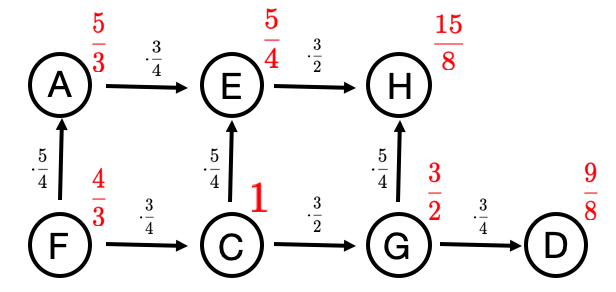
\includegraphics[width=0.7\textwidth]{ScaleLab_15}
\caption*{Just tuning}
\end{figure}

Just Tuning: Let us now consider a tuning that focuses on fifths and thirds. It is called just tuning. For the seven notes in the C major scale it uses the following tuning pattern.

You can play many perfect thirds and fifth with this tuning, but you loose some others. As a matter of fact, this little grid is a small portion of the Tonnetz.


Equal tempered tuning: If you extend both the Pythagorean and the just tuning to all 12 halftones. Some intervals will be perfect, but others won't sound as perfect. The modern approach taken to tuning is to avoid this by equally spreading the error over all intervals. (This might be considered as a kind of democratic approach to tuning). In equal tempered tuning an octave is simply split into 12 equal steps. Each halftone step multiplies the frequency by a factor of $\sqrt[12]{2}$ , which reaches a perfect octave after 12 steps. Using this method, all fifths carry the same error. The same happens for chords and for all other intervals. Let us compare the values of equal tempered tuning to perfect tunings,
$$\textrm{for fifth: } (\sqrt[12]{2})^7 = 1.498\ldots \approx 1.5 = \frac{3}{2} ,$$
$$\textrm{for thirds: } (\sqrt[12]{2})^4 = 1.26\ldots \approx 1.25 = \frac{5}{4} .$$
Note that these approximations are very good.

\paragraph{Experiment:}
Open the tuning box and experiment with different Western tunings. The colors shown in the Tonnetz indicate how close an interval is to a perfect one. It is also very instructive to analyze the different tunings with the ratio tool. It shows the ratios of intervals if they are played on the keyboard. The picture below shows the frequency ratios for a major C chord.

% \begin{figure}[h]
% \centering
% 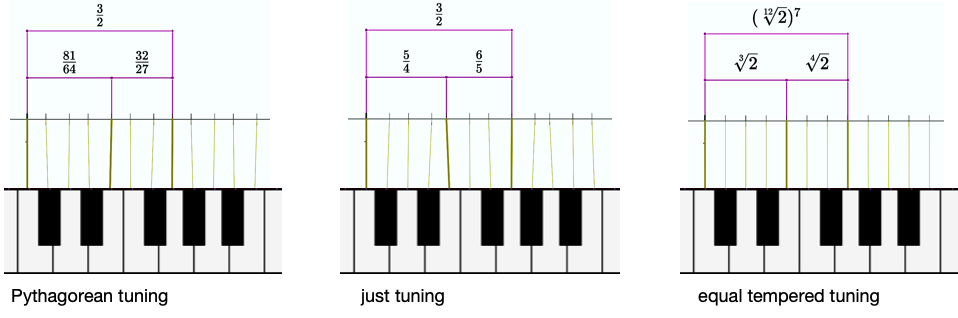
\includegraphics[width=0.95\textwidth]{ScaleLab_18}
% \end{figure}

\begin{figure}[h]
\centering
\begin{tikzpicture}
\scriptsize
\node at (0,0) { 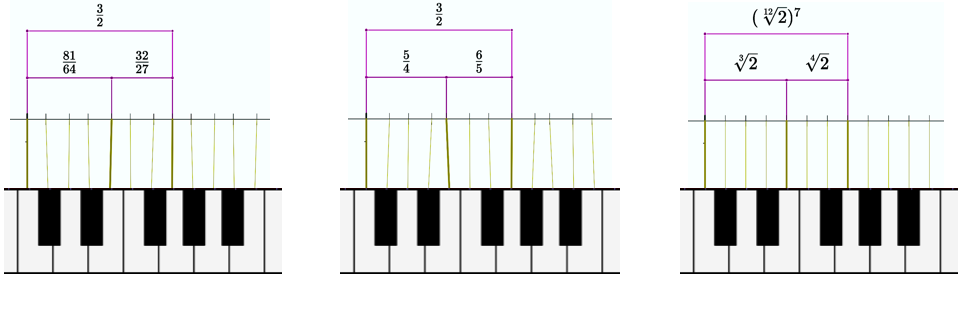
\includegraphics[width=0.95\textwidth]{ScaleLab_18_nolabels} };
\node at (-5.75,-1.65) [align=left, anchor=west]
    {Pythagorean tuning};
\node at (-1.65,-1.65) [align=left, anchor=west]
    {Just tuning};
\node at (2.5,-1.65) [align=left, anchor=west]
    {Equal tempered tuning};
\end{tikzpicture}
\end{figure}

\subsubsection{Indian Raga Scales}
There is another way of playing many perfect fifths and thirds: Add more tones to the scale!  The tuning system for Indian Raga music make utilizes this approach. In short, these tuning systems can be characterized by the following tuning scheme.

\begin{figure}[h]
\centering
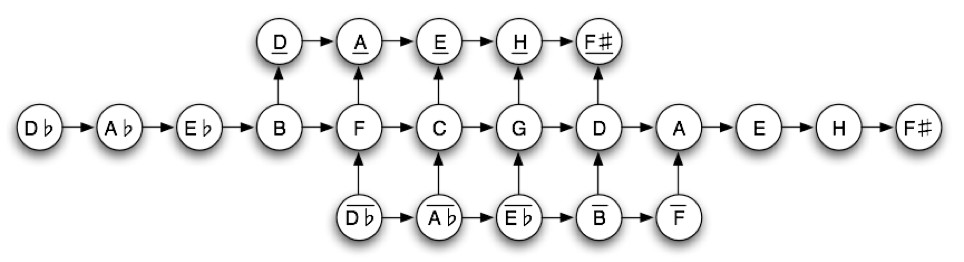
\includegraphics[width=0.9\textwidth]{ScaleLab_19}
\end{figure}


Every horizontal arrow indicates (up to octave jumps) a perfect fifth and every vertical arrow a perfect third. Unlike Western music, Raga music has more an oral than a written tradition. Hence, it is a little difficult to nail down a concrete tuning system but the one described above consisting of 22 tones is accepted among people who analyzed Indian music. What is so special and interesting about this tuning system and why are there exactly 22 tones?

First of all, it should be noted that Indian Ragas always refer to a given base tone. Usually a drone interval is constantly played in the background, the usual one is a C-G sound. Observe how the middle between the C and G is the symmetry center of the above diagram.

The central row of the diagram is the Pythagorean scale with 11 perfect fifths. Now we saturate it by adding perfect thirds, which is done in a very clever way. To see this we reorder the notes of the Pythagorean scale to form a chain of halftones. We get:

\begin{figure}[h]
\centering
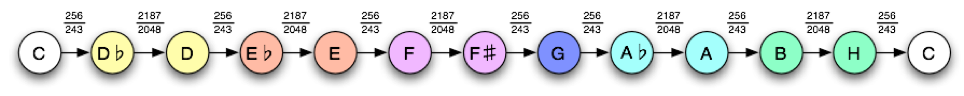
\includegraphics[width=0.95\textwidth]{ScaleLab_21}
\end{figure}

The ratios between the tones represent the frequency ratios that come from the Pythagorean tuning.

You can see that, almost magically, only two kinds of fractions occur. The coloring in the diagram marks the bigger of the two fractions, thus we have big halftone steps and small halftone steps. Two tones that are related by a big step have the same color. Now one can split the interval of 2187/2048 in an elegant way by introducing two new notes.

\begin{figure}[h]
\centering
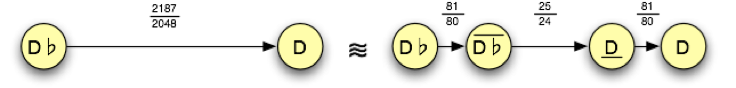
\includegraphics[width=0.95\textwidth]{ScaleLab_22}
\end{figure}

In the example above you additionally get a higher version of the D$\flat$   and a lower version of the D. These are exactly the two versions added in the above tone system. We can now do a similar split for all other big halftone steps. This results in the system with 22 tones, shown in the following colored version of this tone system:

\begin{figure}[h]
\centering
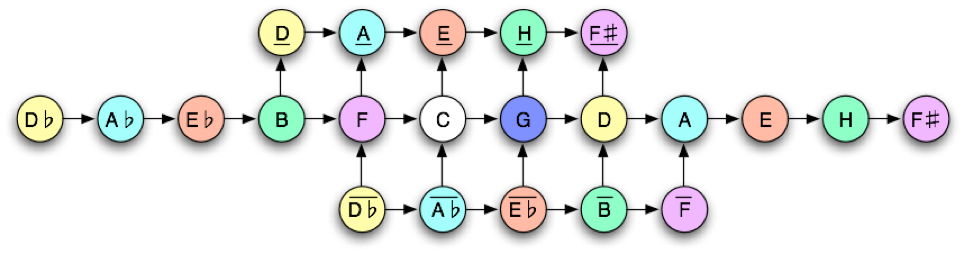
\includegraphics[width=0.95\textwidth]{ScaleLab_20}
\end{figure}

Notice that the C and G play a special role in this system as the only notes that are not involved in a split interval.

The tones of the Raga tuning system are called Shrutis. As in the Western tuning systems, often a melody does not make use of all tones at the same time. Instead, certain notes are selected to form smaller scales based on the bigger tone system. Also the selection of sub scales (usually of four to seven tones) follows certain rules. But we will not go into those details here.

\paragraph{Experiment:} Open the tuning box and experiment with the sounds of the Raga tunings. You can start the drone tone and select among plenty of commonly used sub scales of the 22 tone system. It might also be interesting to measure frequency ratios between the tones.

\begin{sectcredits}
\item[Author of this exhibit:] Jürgen Richter-Gebert (Technical University of Munich)
\item[Acknowledgements:] Patrick Wilson and Aaron Montag (Sound Engine). Based on CindyJS.org
\item[Text:] Jürgen Richter-Gebert (TU Munich)
\end{sectcredits}
